\chapter{Lanczos Filter}\label{ap01}

\section{Formulation}

The Lanczos band-pass filter is mathematically formulated as follows:

\begin{equation}
w(n) = 
\begin{cases} 
2 \cdot (\text{cutoff}_\text{high} - \text{cutoff}_\text{low}) & \text{if } n = 0 \\
\left( \text{sinc}(2 \cdot \text{cutoff}_\text{high} \cdot n) - \text{sinc}(2 \cdot \text{cutoff}_\text{low} \cdot n) \right) \cdot \text{sinc}\left(\frac{n}{N}\right) & \text{if } n \neq 0 
\end{cases}
\end{equation}

where $n$ is the index of the weight in the filter window, $w(n)$ is the weight at index $n$, $\text{cutoff}_\text{low}$ and $\text{cutoff}_\text{high}$ are the specified lower and upper cutoff frequencies, respectively, and $N$ is half the length of the filter window. The $sinc$ function is defined as:

\begin{equation}
\text{sinc}(x) = \frac{\sin(\pi x)}{\pi x}
\end{equation}

\section{Related Issues}

The Lanczos filter, like other finite impulse response filters (FIR), can exhibit issues at discontinuities in the data. For the vorticity data series, this would be at its endpoints. These issues arise primarily due to the Gibbs phenomenon and edge effects:

1. \textbf{Gibbs Phenomenon}: The Gibbs phenomenon refers to the overshoot and ringing that occurs near discontinuities when approximating a function with a finite series of basis functions \citep{gibbs1898, hamming1989}. In the context of the Lanczos filter, which utilizes a sinc function, abrupt changes at the edges of the filter window can cause ringing effects at the points of discontinuity in the data.

2. \textbf{Edge Effects}: FIR filters, including the Lanczos filter, can produce artifacts at the boundaries of the data series due to the reliance on data points that may not be available at the edges \citep{oppenheim2009, proakis2006}. Techniques such as zero-padding or reflection are often used to mitigate these effects, but they can still result in artifacts or less accurate filtering near the boundaries.

3. \textbf{Finite Window Length}: The window length of the Lanczos filter determines the number of data points used in the convolution. A finite window length means the filter may not fully capture long-term trends or low-frequency components, especially at the edges, leading to discontinuities or spurious oscillations \citep{smith1997, oppenheim1999discrete}.

4. \textbf{Windowing Effect}: The Lanczos filter uses a windowed $sinc$ function to perform the convolution. While windowing reduces spectral leakage by smoothing the transition at the edges of the filter, it also introduces artifacts, particularly near discontinuities where the transition from one region to another is abrupt \citep{harris1978, mitra2001}.

To mitigate this, a weaker low-pass Lanczos filter is applied to the initial and final 5\% of the data series, ensuring smoother transitions at the endpoints (Figure \ref{fig:/cyclophaser_methodology}b).

\chapter{Lorenz Energy Cycle Program Description}\label{ap02}

To compute the Lorenz Energy Cycle (LEC), an open-source Python application named "lorenz-cycle" was developed and is available on GitHub. The application is designed for collaboration and transparency, allowing peers to freely use, modify, and review the computation procedures. Full documentation and a user guide with illustrative examples can be found at \url{https://github.com/daniloceano/lorenz-cycle}. 

The lorenz-cycle application utilizes the mathematical expressions detailed in Section \ref{math} and supports both Eulerian and Semi-Lagrangian frameworks. Additionally, it can compute the generation and dissipation terms directly or estimate them as residuals. When using the residual approach, the budget equations are estimated using finite differences: a first-order forward/backward method is applied to the endpoints, while second-order centered differences are employed for the remaining data points. Regardless of whether residuals are estimated or not, the generation terms are always computed.

In the Semi-Lagrangian framework, users can either run the program using a predefined track file or iteratively choose the computation domain step-by-step. For the Eulerian framework, users must provide a "box limits" file containing the minimum and maximum latitudes and longitudes for the desired computational domain. When using a predefined track file, the track may only contain the system's central position (latitude and longitude), in which case the program defaults to a $15^\circ \times 15^\circ$ domain for each time step. The track file can also be adjusted to include the length and width of the computational domain for each time step.

Additionally, in the Semi-Lagrangian approach, users can provide an input file containing the required meteorological data or, by using an appropriate program flag, automatically download the matching ERA5 dataset using ECMWF's Python plugin "CDS API" (\url{https://pypi.org/project/cdsapi/}). To use this option, the user must install and configure the library as instructed at \url{https://cds.climate.copernicus.eu/api-how-to}.

The program is not limited to the ERA5 dataset and can run with any meteorological dataset, whether it is reanalysis data or model output. It reads a namelist file specifying the variable naming conventions used in the input file. The requirements for the input file are: 1) it must be a NetCDF file, 2) the horizontal grid must be structured, and 3) it must use an isobaric vertical coordinate system. The file should also contain data for temperature, u and v wind components, $\omega$ vertical wind component, and either geopotential or geopotential height data.

For handling meteorological constants and variable units, the lorenz-cycle program uses the MetPy package \citep{may2022metpy}. This open-source package, initially developed and maintained by the National Science Foundation (NSF) Unidata, a member of the University Corporation for Atmospheric Research (UCAR) Community Programs, ensures correct variable assignment and unit conversion, preventing errors such as summing variables with different units.

To ensure efficient and fast computations, the program is fully parallelized using Dask, a parallel computing library that handles large datasets efficiently \citep{daniel2019data}. Dask allows large data arrays to be split into smaller chunks for independent processing by multiple computing cores, preventing memory overload and optimizing performance. In the lorenz-cycle program, Dask's configuration is optimized to handle large matrices by dividing them into smaller chunks for efficient processing.

The program outputs the results for each term in comma-separated values (CSV) files. It generates one CSV file for each term, and for energy, conversion, and generation terms, it also provides results for each vertical level, enabling a two-dimensional analysis. Additionally, the program can be configured by the user to automatically generate plots. These plots include spatial representations of the computational domain defined for the analysis, time series of the system's central minimum pressure and relative vorticity at 850 hPa, time series of each LEC term, Hovmöller diagrams, and complete energy flux boxes for the LEC.

\chapter{Complete Life Cycle LEC EOFs Reconstructed}\label{ap03}

Figures \ref{fig:ap_eofs} illustrate the reconstructed EOFs for the complete life cycle. These EOFs were reconstructed by reversing the normalization process and adding the mean values to each EOF.

\begin{figure}[!htbp]
\centering
\begin{tabular}{cc}
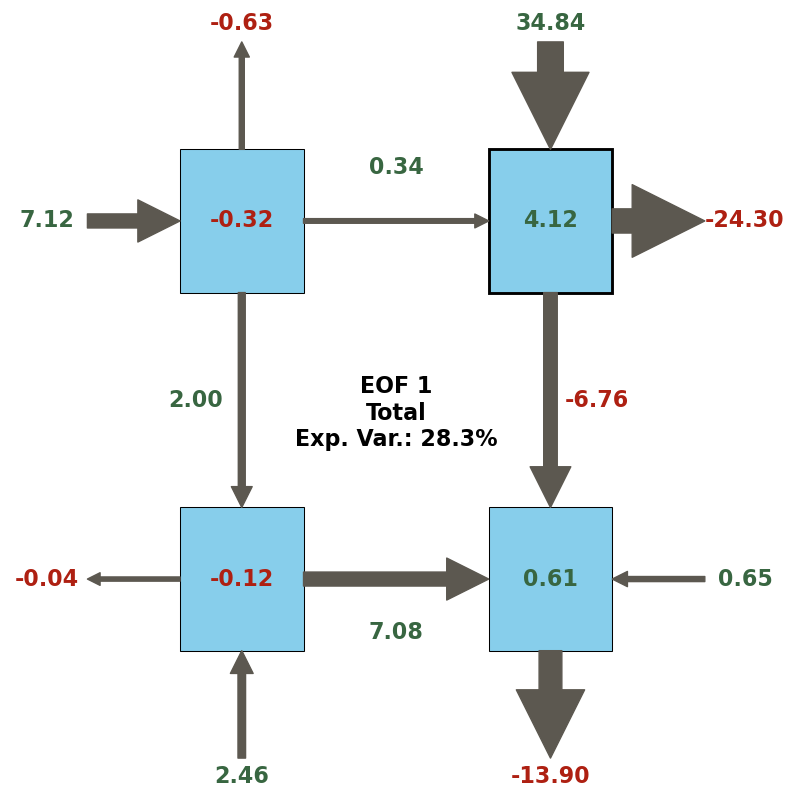
\includegraphics[width=0.46\textwidth]{figs_appendix/Total_eof1_with_mean.png} & 
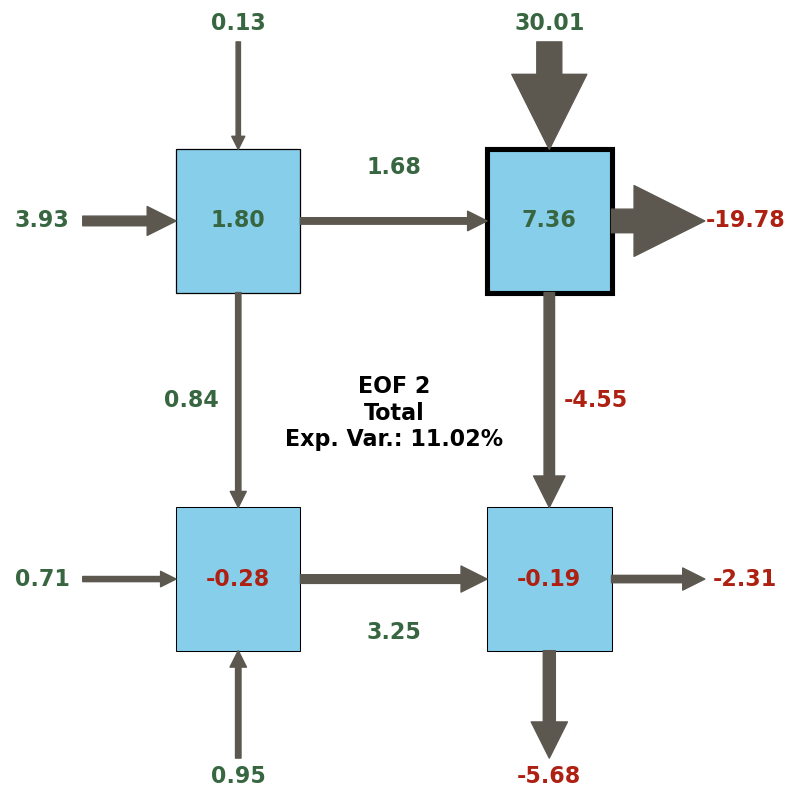
\includegraphics[width=0.46\textwidth]{figs_appendix/Total_eof2_with_mean.png} \\
(a) Reconstructed EOF1 & (b) Reconstructed EOF2 \\
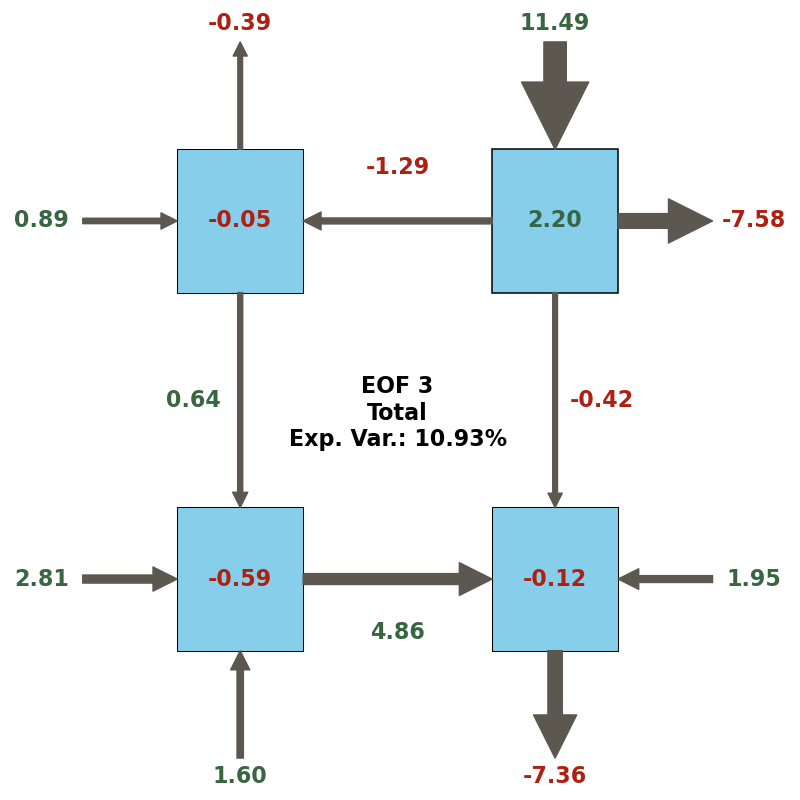
\includegraphics[width=0.46\textwidth]{figs_appendix/Total_eof3_with_mean.png} & 
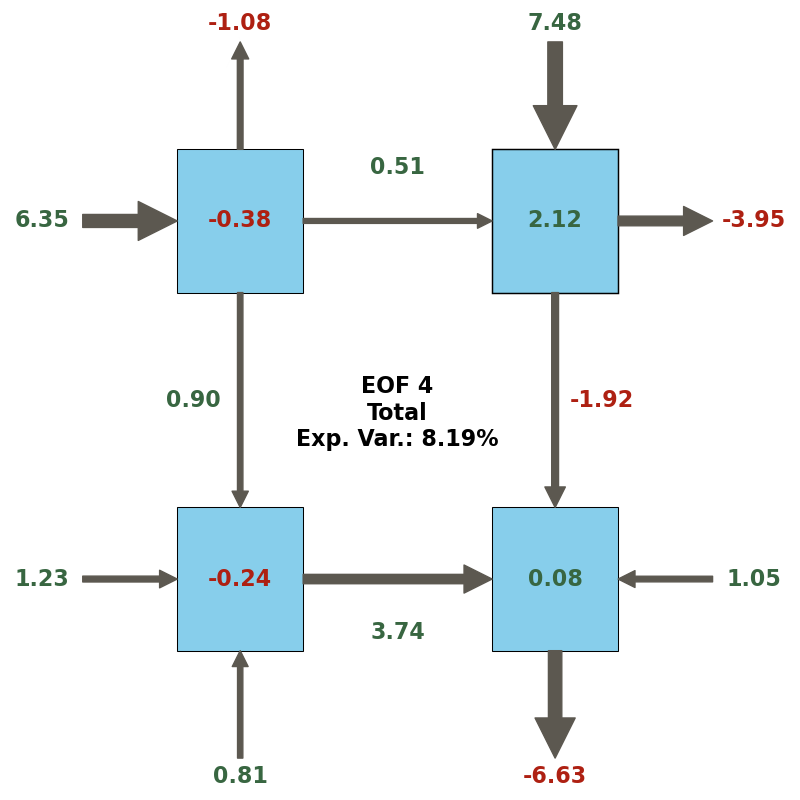
\includegraphics[width=0.46\textwidth]{figs_appendix/Total_eof4_with_mean.png} \\
(c) Reconstructed EOF3 & (d) Reconstructed EOF4 \\
\end{tabular}
\caption[Reconstructed EOFs]{Lorenz Energy Cycle (LEC) Terms EOFs reconstructed. The numbers adjacent to the arrows denote the magnitude and direction of the anomaly, with green indicating positive values and red indicating negative values.}
\label{fig:ap_eofs}
\end{figure}

\chapter{LEC - Terms Correlation}\label{ap04}

Figure \ref{fig:ap04} presents correlation plots between the conversion terms $C_A$ and $C_E$ (Figure \ref{fig:ap04}a) and between eddy kinetic energy $K_E$ and relative vorticity at 850 hPa in the cyclone center (Figure \ref{fig:ap04}b).

\begin{figure}[!htbp]
\centering
\begin{tabular}{cc}
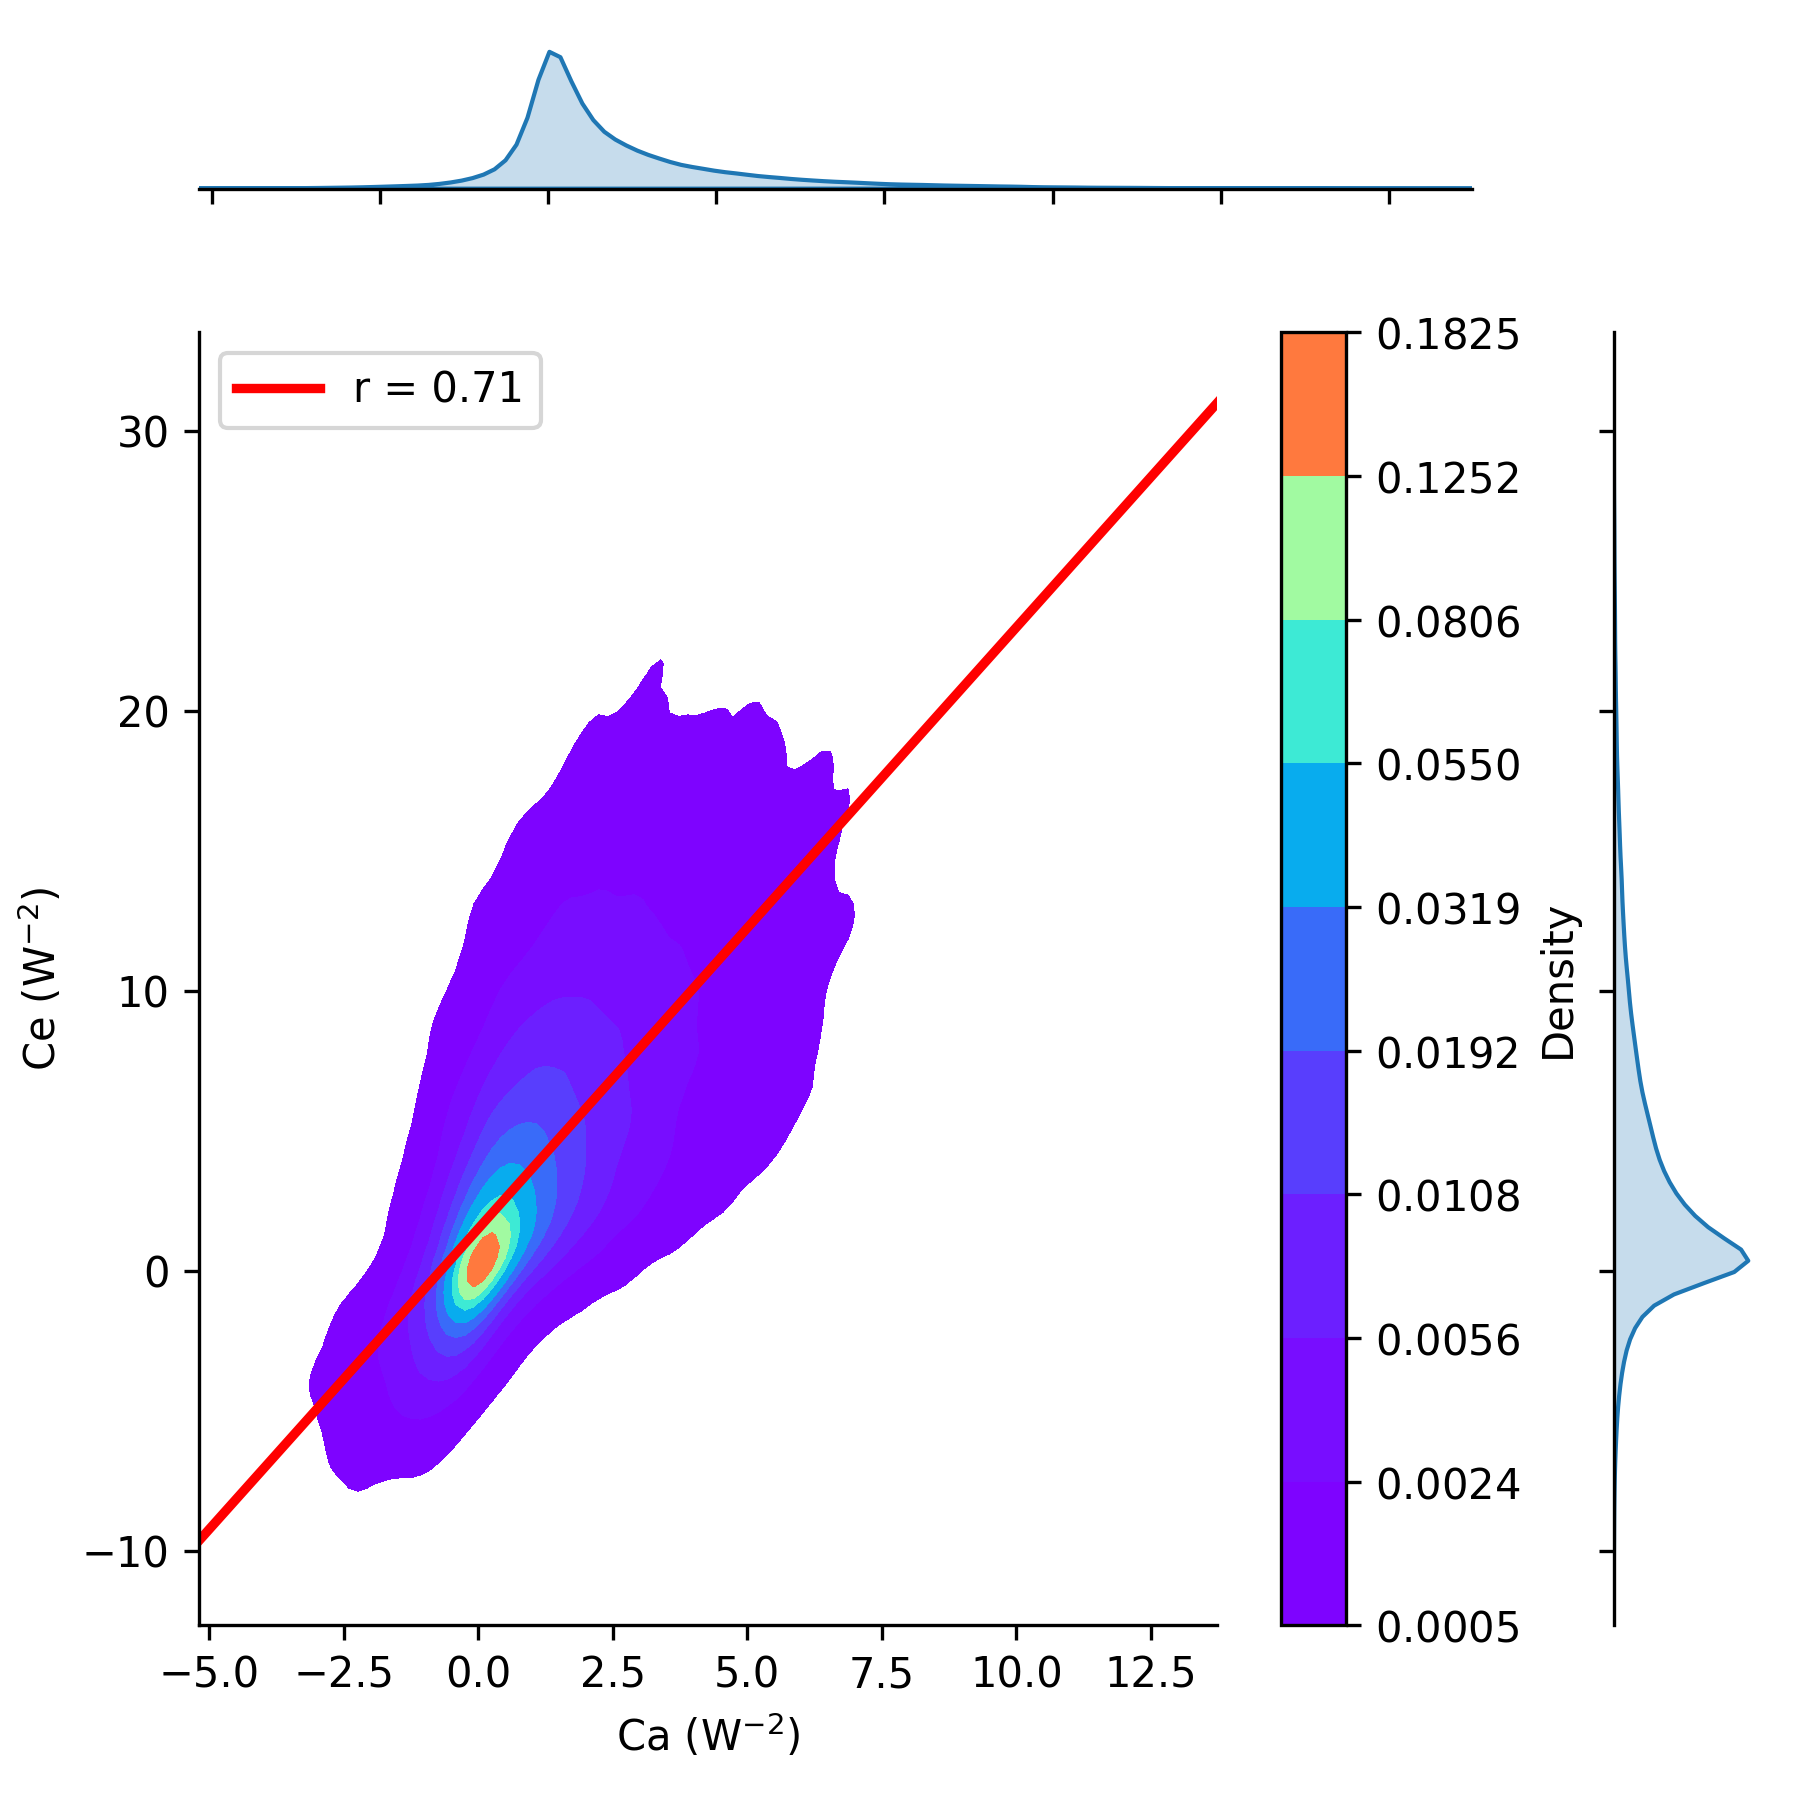
\includegraphics[width=0.46\textwidth]{figs_appendix/correlation_ca_ce.png} & 
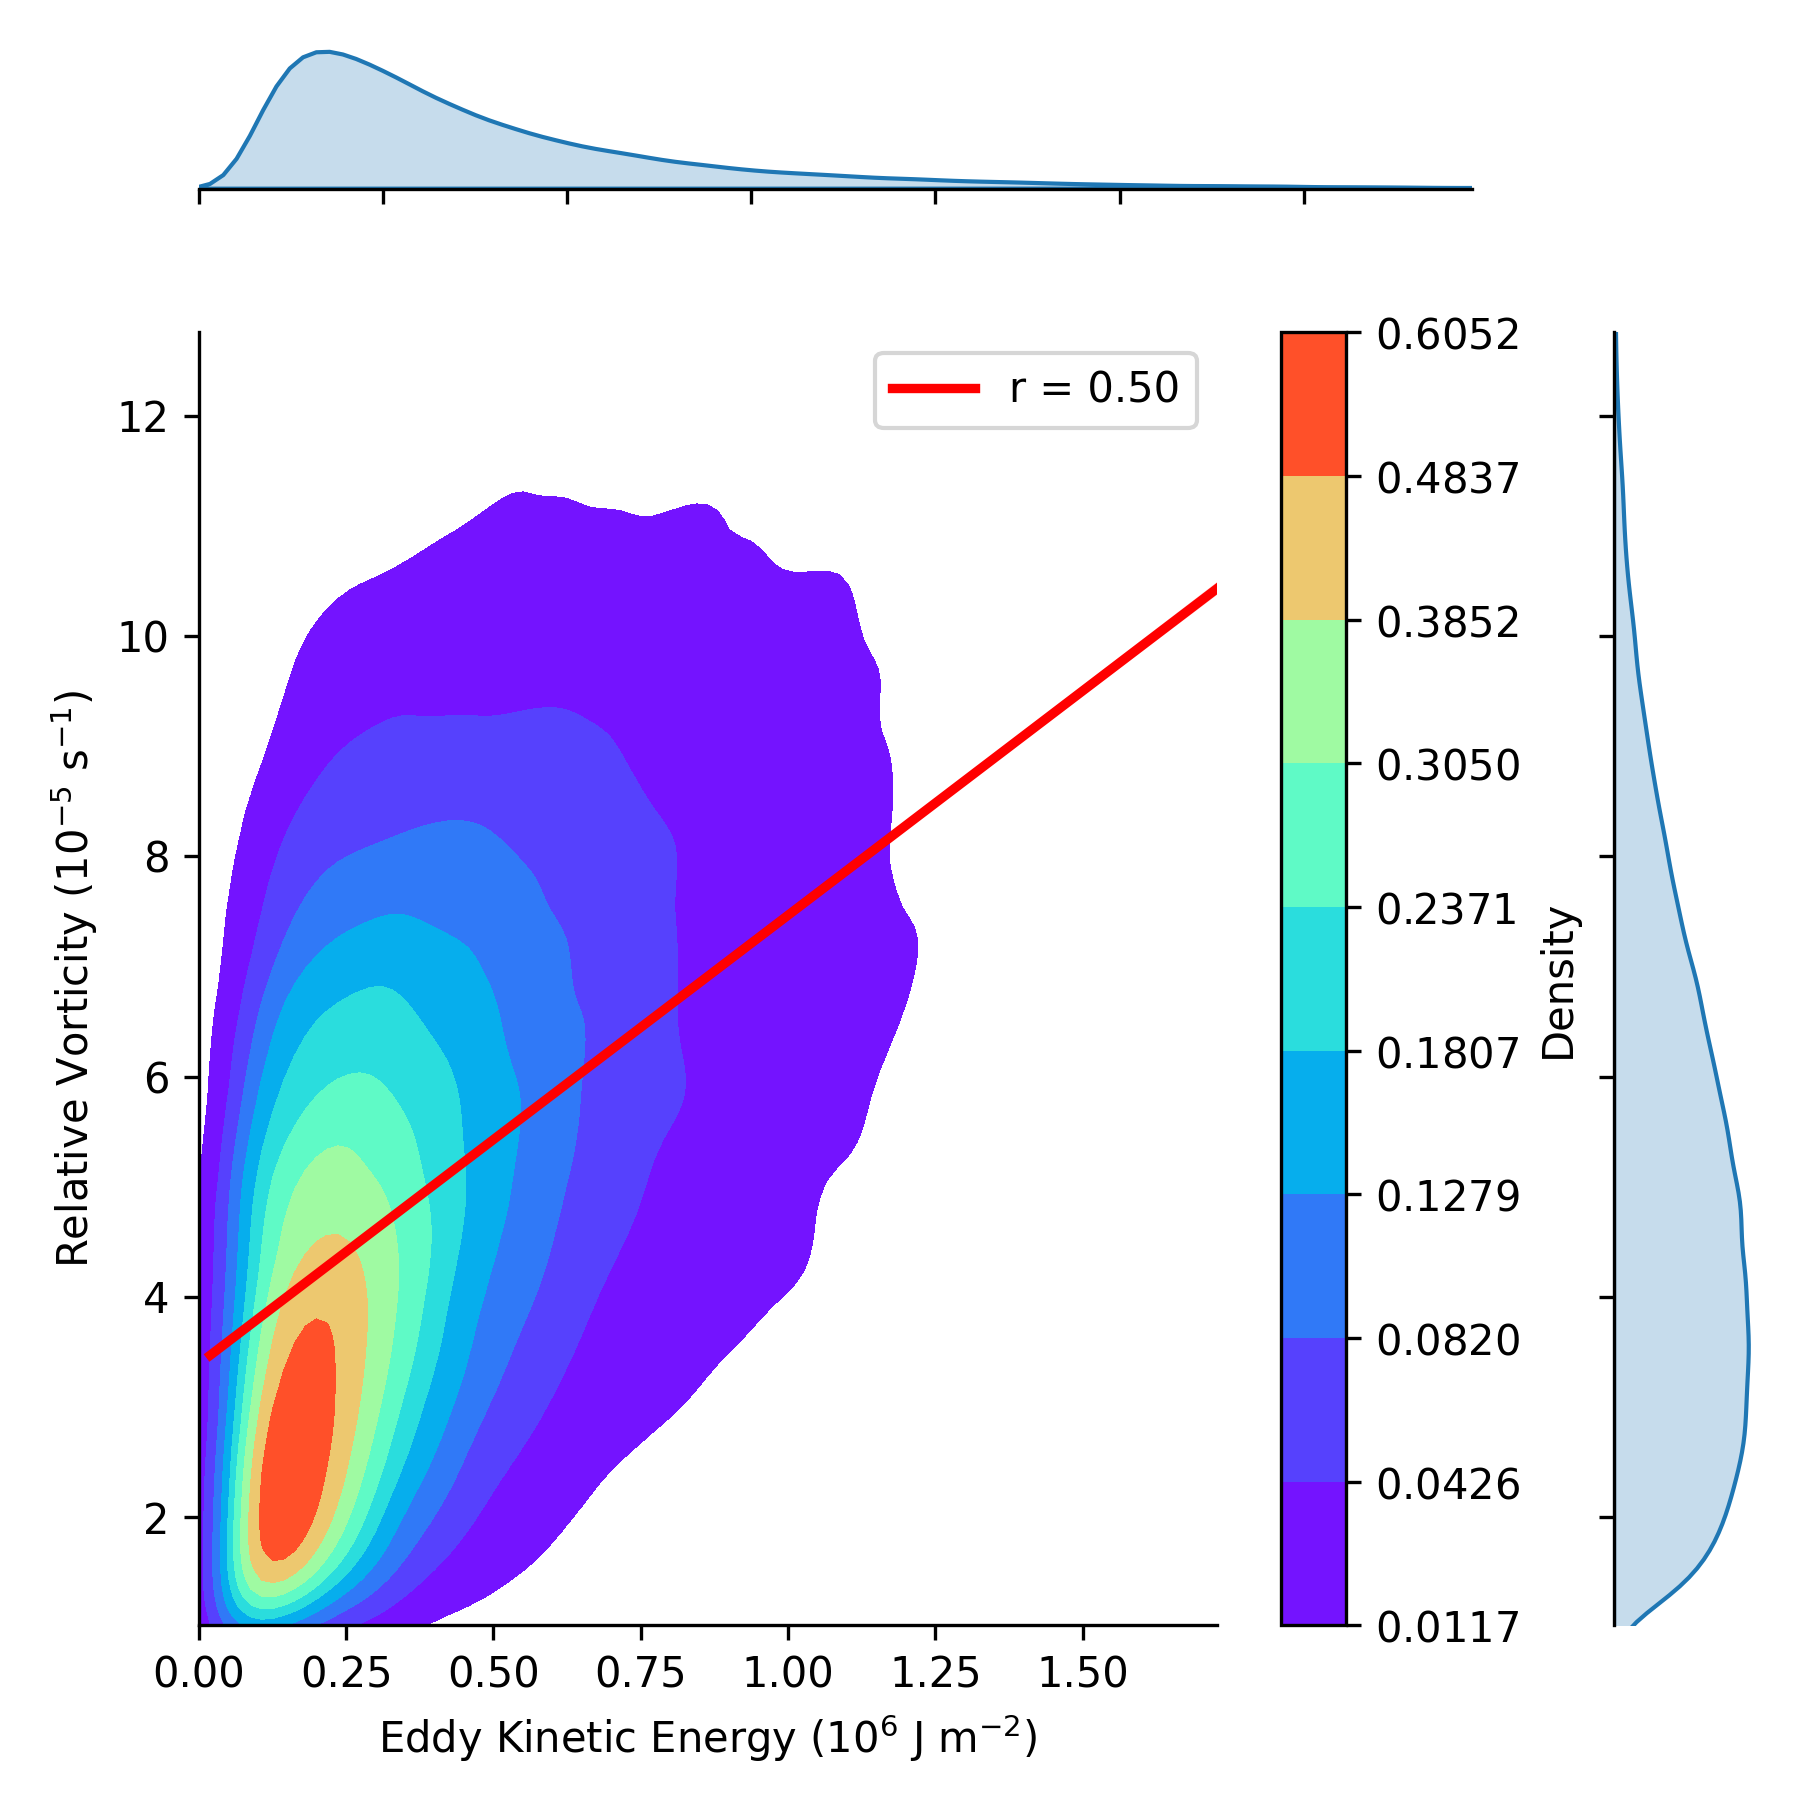
\includegraphics[width=0.46\textwidth]{figs_appendix/correlation_ke_vor42.png} \\
(a) & (b) \\
\end{tabular}
\caption[Correlation Between LEC Terms]{Correlation between $C_A$ and $C_E$ (a), as well as between $K_E$ and relative vorticity at 850 hPa in the cyclone center (b). The red line represents the linear regression, with the Pearson's correlation coefficient (r) indicated in each plot.}
\label{fig:ap04}
\end{figure}

\chapter{LEC Results for Reg1 System}\label{ap05}

Here, the same analysis conducted by \citet{dias2011energy} is performed for the "Reg1" system. The aim is to validate the results obtained by the "lorenz-cycle" program and provide support for the analysis performed using the Lorenz Phase Space Diagrams. Figure \ref{fig:box_limits_reg1} illustrates the computational domain used for computing the LEC for this system, while Figure \ref{fig:energy_conversion_timeseries_reg1} displays the energy and conversion terms, matching Figure 5 from \citet{dias2011energy}.

\begin{figure}[!htbp]
\centering
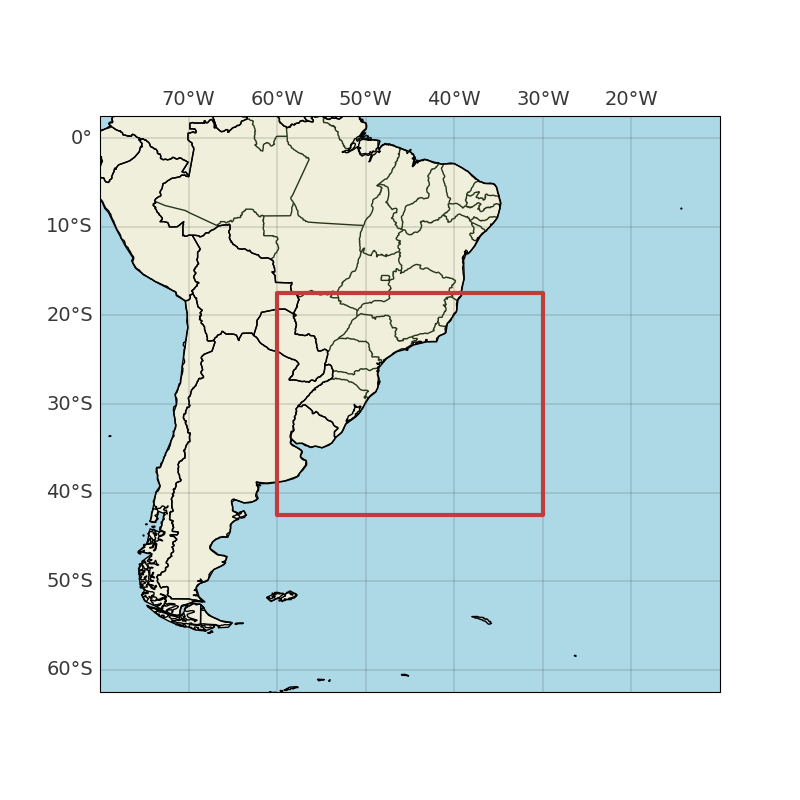
\includegraphics[width=0.46\textwidth]{figs_appendix/box_limits.png}
\caption[Computational Domain - Reg1 System]{Computational domain used for analyzing the "Reg1" system \citep{dias2011energy}.}
\label{fig:box_limits_reg1}
\end{figure}

\begin{figure}[!htbp]
\centering
\begin{tabular}{cc}
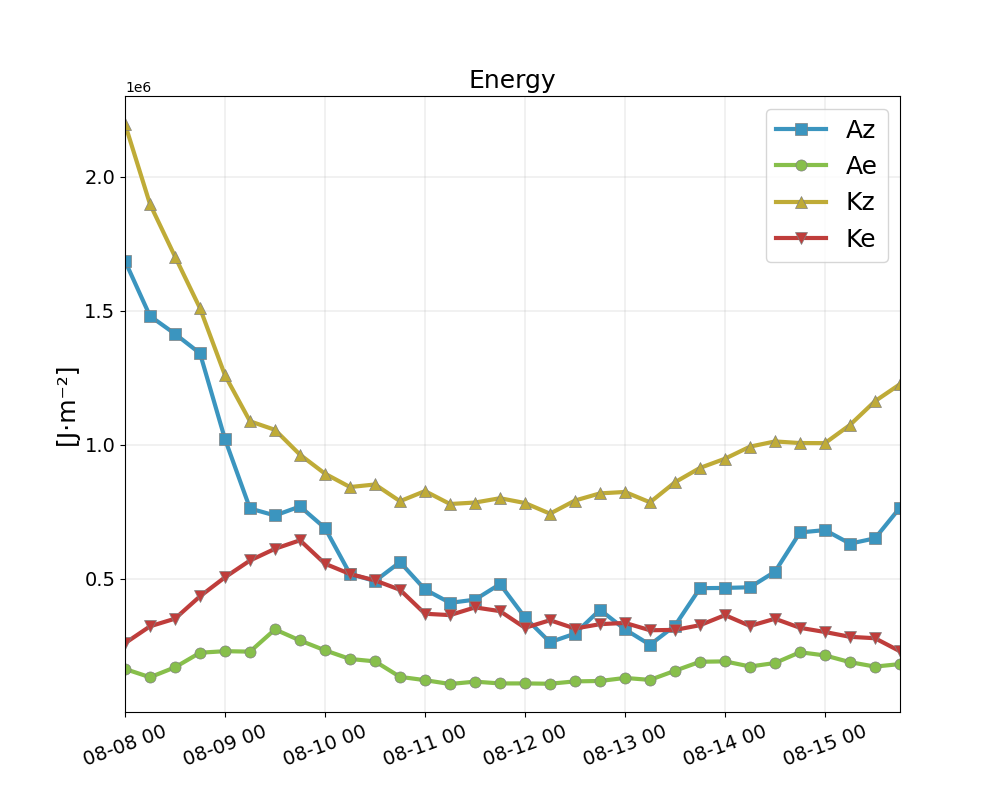
\includegraphics[width=0.46\textwidth]{figs_appendix/timeseires_energy.png} & 
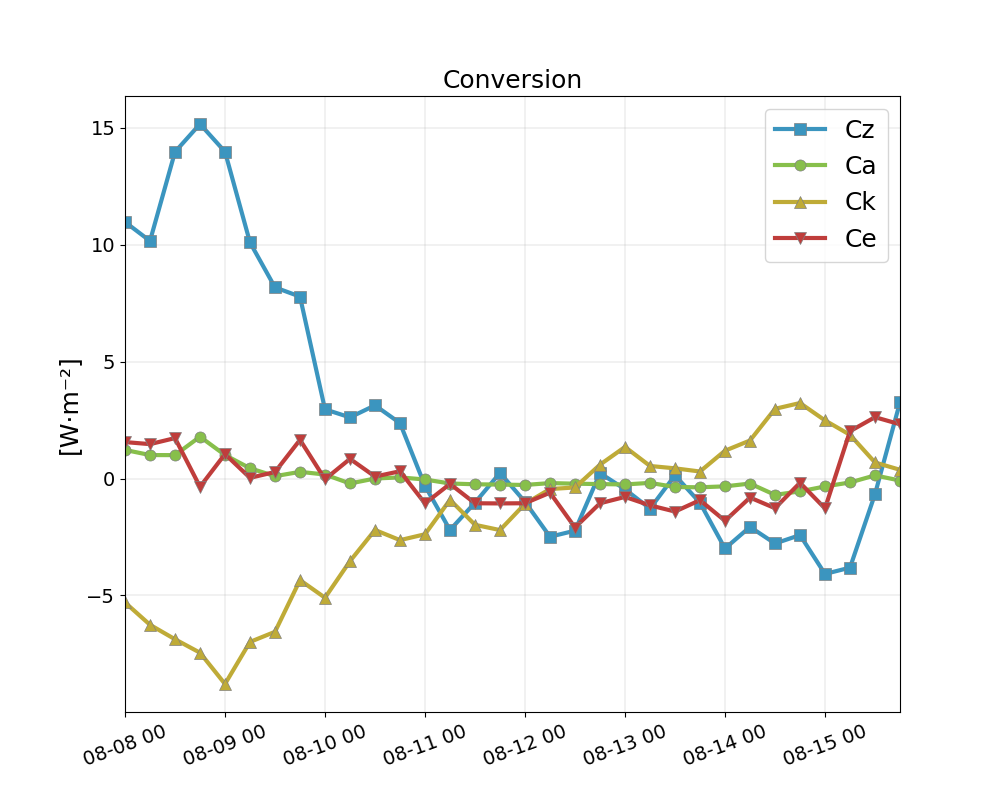
\includegraphics[width=0.46\textwidth]{figs_appendix/timeseires_conversion.png} \\
\end{tabular}
\caption[Energy and Conversion Terms - Reg1 System]{Energy and conversion terms computed for the "Reg1" system \citep{dias2011energy}, using an Eulerian framework (Figure \ref{fig:box_limits_reg1}).}
\label{fig:energy_conversion_timeseries_reg1}
\end{figure}

\chapter{Lorenz Phase Space - All Systems}\label{ap:06}

Figures \ref{fig:lps_1_all_systems} and \ref{fig:lps_2_all_systems} illustrate the LPS diagrams for all systems with genesis in ARG, LA-PLATA, and SE-BR between 1979 and 2020. Due to the large amount of data and the presence of outliers, it is not possible to discern the relative importance of the LEC terms for smaller groups of systems precisely. However, the LPS visualization still provides an overview of the main mechanisms related to cyclone development in the SESA region.

For LPS diagram type 1, a cloud of data spreads primarily over the top-left quadrant. Moreover, there is a high density below the 1:1 diagonal line. This indicates that for most systems, there is a shared importance of baroclinic and barotropic conversions for eddy development, as indicated in previous chapters. For diagram type 2, a clear distinct tendency cannot be found from this analysis, indicating a high quantity of systems that either import or export both $A_E$ and $K_E$.


\begin{figure}[!htbp]
\centering
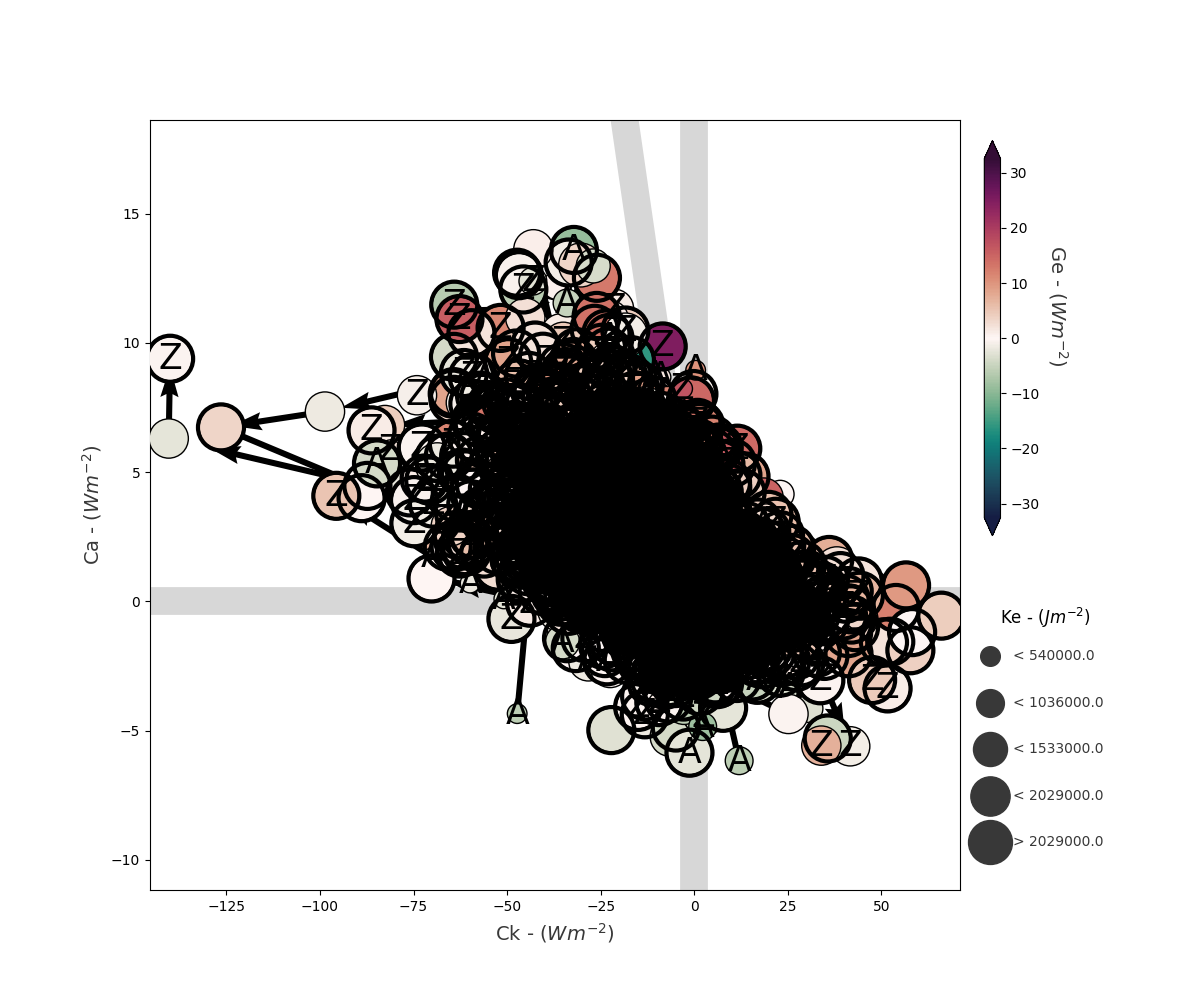
\includegraphics[width=\textwidth]{figs_6/lps_mixed_all_systems_zoom.png}
\caption[LPS 1 - All Systems]{Lorenz Phase Space (LPS) diagram 1 for all systems with genesis near South America.}
\label{fig:lps_1_all_systems}
\end{figure}

\begin{figure}[!htbp]
\centering
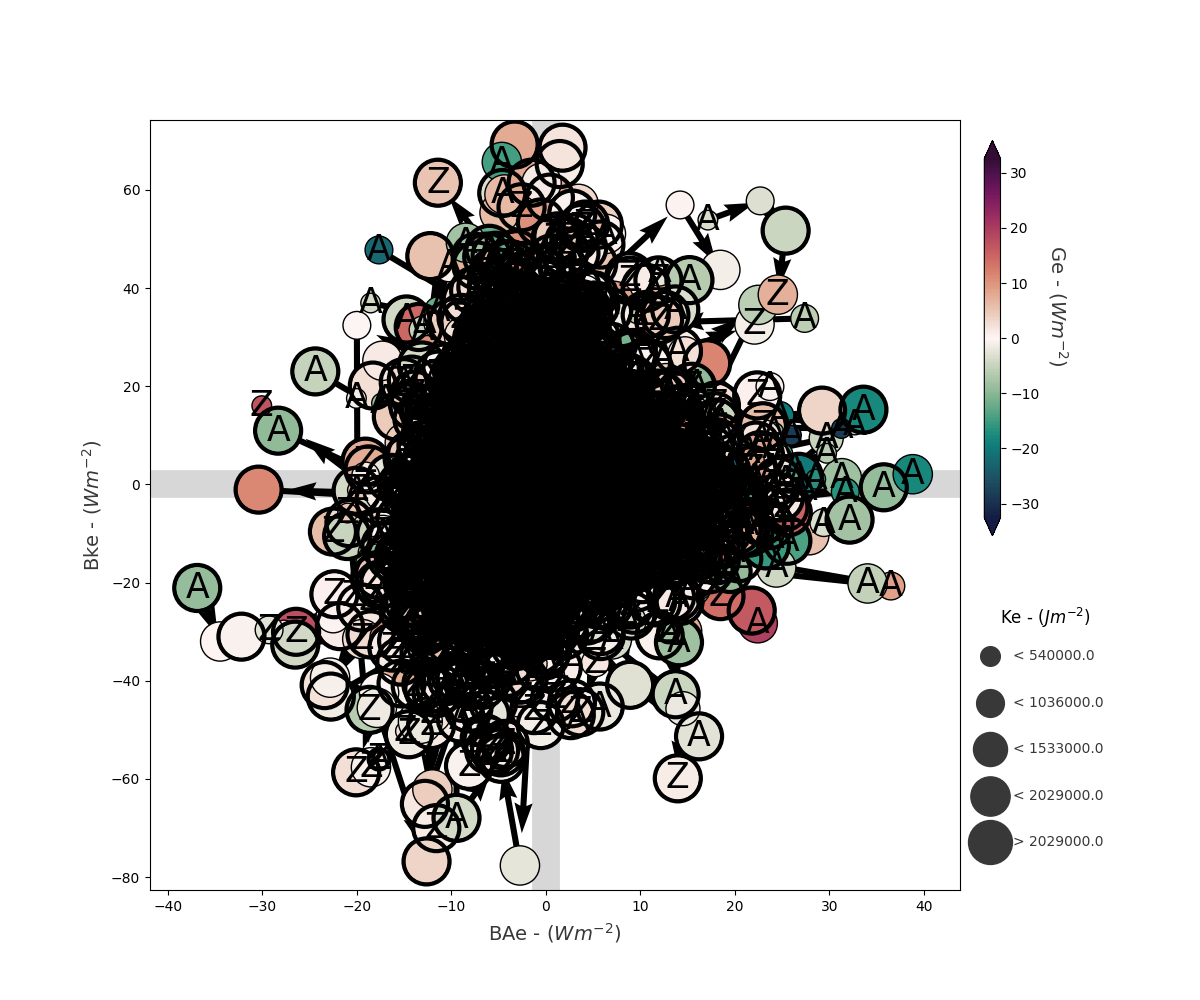
\includegraphics[width=\textwidth]{figs_6/lps_imports_all_systems_zoom.png}
\caption[LPS 1 - All Systems]{Lorenz Phase Space (LPS) diagram 2 for all systems with genesis near South America.}
\label{fig:lps_2_all_systems}
\end{figure}

\chapter{Lorenz Phase Space 1 - Early Decay}\label{ap:07}

\begin{figure}[!htbp]
\centering
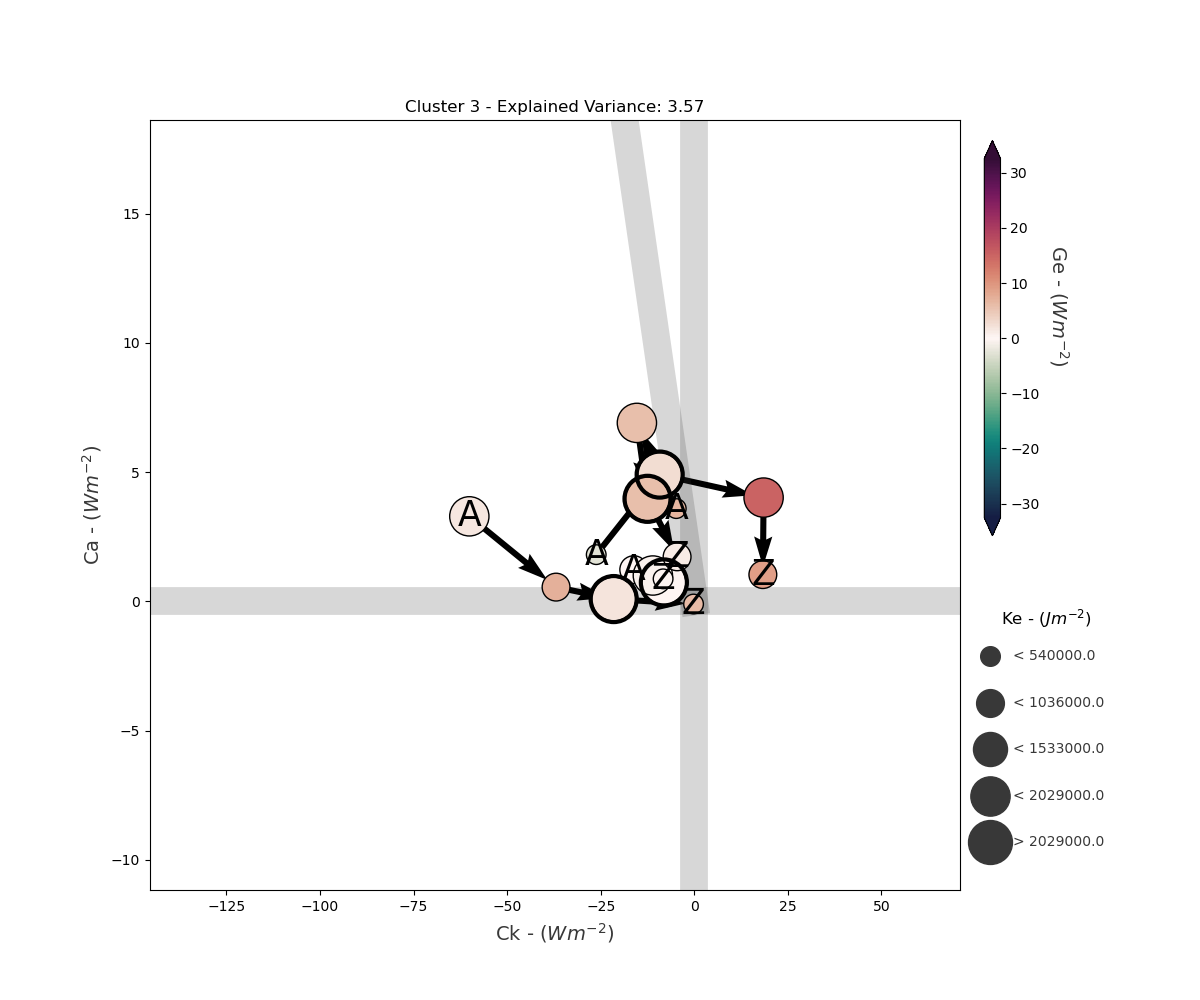
\includegraphics[width=\textwidth]{figs_appendix/lps_mixed_cluster_3_all_systems.png}
\caption[LPS 1 - Cluster 3 - DItMD]{Lorenz Phase Space (LPS) diagram 1 for all systems represented in cluster 3 of the "decay, intensification, matude, decay 2" life cycle.}
\label{fig:lps_mixed_cluster_3_all_systems}
\end{figure}

\chapter{Lorenz Phase Space - Most Intense Systems}\label{ap:08}

\begin{figure}[!htbp]
\centering
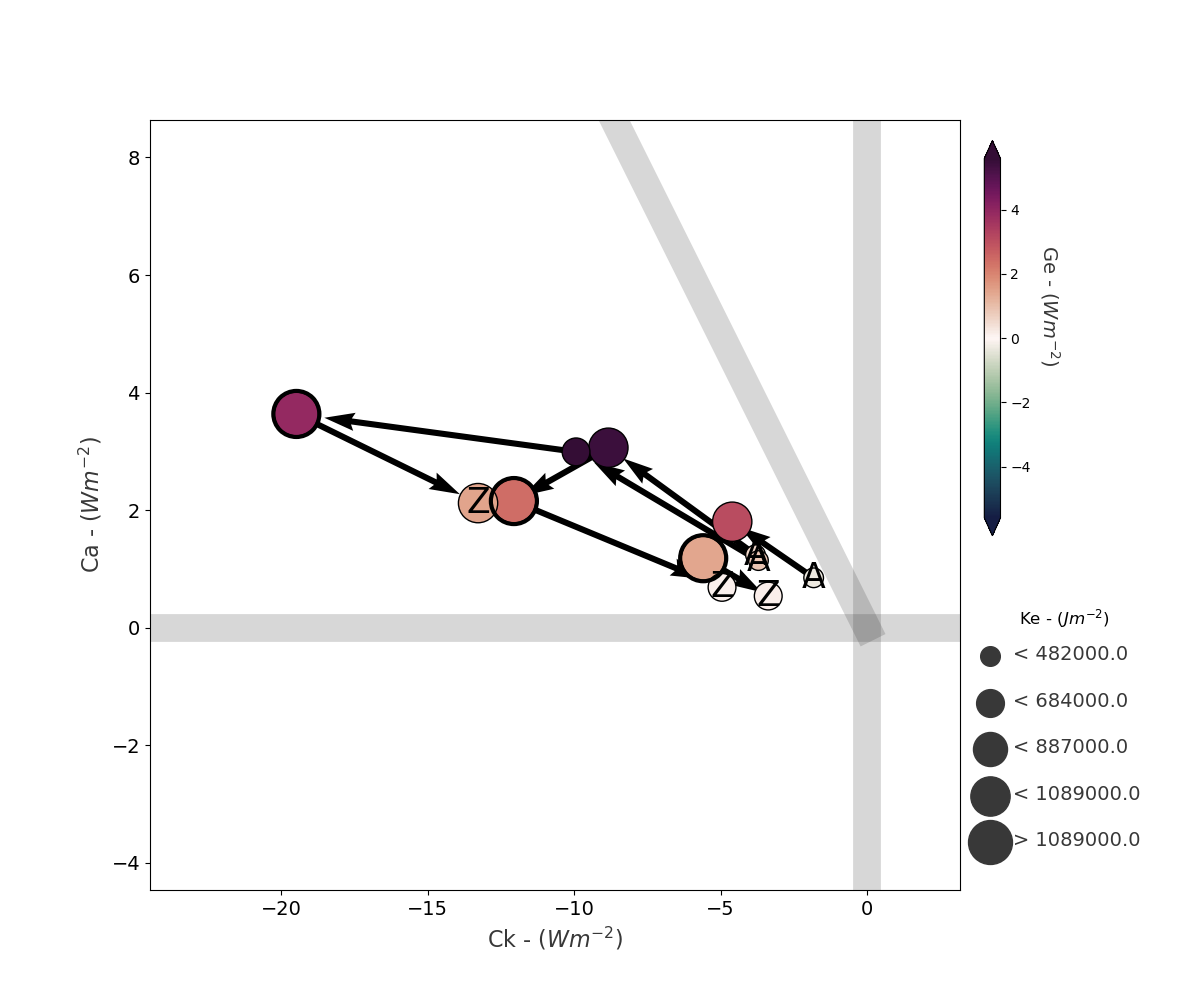
\includegraphics[width=\textwidth]{figs_appendix/lps_mixed_all_systems_all_clusters_zoom.png}
\caption[LPS 1 - Most Intense Systems]{Lorenz Phase Space (LPS) diagram 1 for the energy patterns of the systems presenting central relative vorticity higher than the 0.9 quantile.}
\label{fig:lps_mixed_all_systems_all_clusters_zoom}
\end{figure}

\chapter{Tracks - Energy Pattern 1}\label{ap:09}

\begin{figure}[!htbp]
\centering
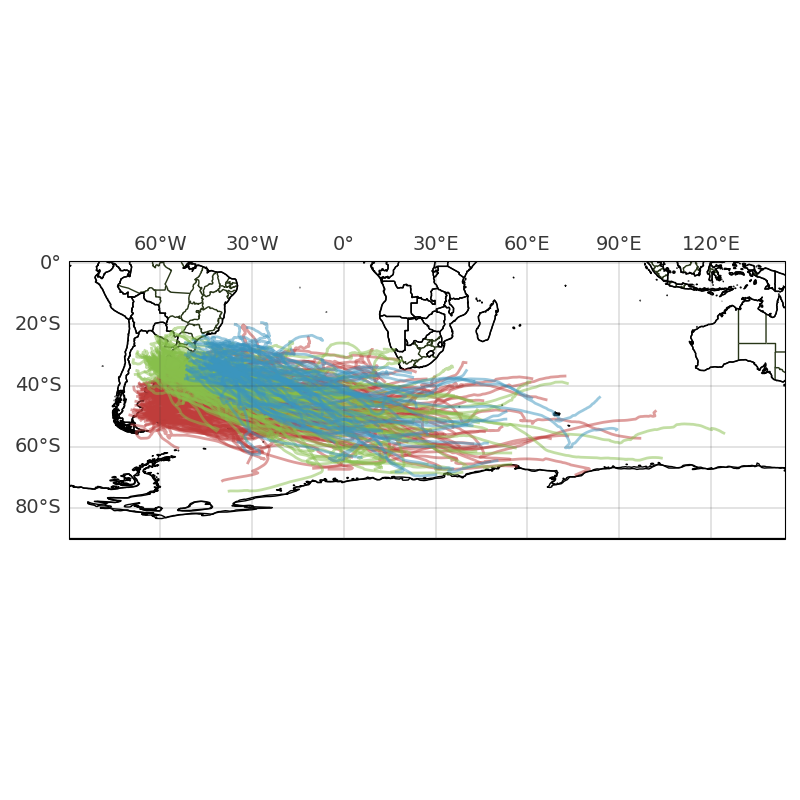
\includegraphics[width=\textwidth]{figs_appendix/tracks.png}
\caption[Tracks - EP1]{Cyclone tracks associated with energy pattern (EP) 1.}
\label{fig:tracks_ep1}
\end{figure}